\documentclass[conference]{IEEEtran}
\IEEEoverridecommandlockouts
% The preceding line is only needed to identify funding in the first footnote. If that is unneeded, please comment it out.
\usepackage{cite}
\usepackage{amsmath,amssymb,amsfonts}
\usepackage{algorithmic}
\usepackage{graphicx}
\usepackage{subcaption}
\usepackage{textcomp}
\usepackage{xcolor}
\usepackage{authblk}
\usepackage{booktabs}
\usepackage{tabularx}
\usepackage{array}
\usepackage{makecell}
\usepackage{lipsum}
\usepackage{etoolbox}
\def\BibTeX{{\rm B\kern-.05em{\sc i\kern-.025em b}\kern-.08em
    T\kern-.1667em\lower.7ex\hbox{E}\kern-.125emX}}
\makeatletter
\patchcmd{\@maketitle}{\raggedright}{\centering}{}{}
\patchcmd{\@maketitle}{\raggedright}{\centering}{}{}
\makeatother

\begin{document}

\title{Social Distance Detection Using YOLO\\
{}
}
\author{Ashok V}
\affil{Post Graduate Student in Computer Science}
\affil{Government Model Engineering College Kochi, Kerala, India}

\maketitle

\begin{abstract}
The world has been facing a unique situation for the past two years, COVID-19. It reached every corner of the world. There are different methods to prevent the spread. Usage of masks, avoiding social gatherings, washing your hands, maintaining social distancing, etc. Maintaining social distance is the best strategy to prevent the spread of the virus. But people do not care about social distancing. It causes the further spread of the virus. The goal of social distancing is to keep healthy people and those who are sick from coming into close contact with one another. It slows down the spread of the virus. It is very difficult to monitor social distancing in public places. But by using technologies like machine learning, deep learning, and computer vision, it is possible to monitor social distancing automatically. This paper proposes a method in which the video frame from the camera is used as input and the open source object detection pre-trained model based on the YOLO-v4 algorithm is employed for detection of people. Then the distance between people is estimated. The pair that violates the social distancing will be highlighted red. With the help of YOLO, real-time detection is possible. 
\end{abstract}

\begin{IEEEkeywords}
COVID-19, YOLO, deep learning
\end{IEEEkeywords}
\section{Introduction}
COVID-19 has rapidly affected our daily life, global economy, business, etc. The virus is spreading rapidly across the world. Most of the companies are stopped their manufacturing processes, software companies are started work from home culture , classes in schools and colleges are happening in online mode the world is changed in different way. All these changes are due to a small virus called Corona virus. 
\par 
COVID-19 also known as corona virus disease 2019 is a disease which is caused by the severe acute respiratory syndrome conronavirus 2 (SARS-CoV-2). The virus is first reported at Wuhan, China in the month of December 2019. It is spread worldwide, leading to a pandemic. The most common symtoms of the COVID-19 disease are fever, cough, headache, fatigue, breathing difficulties, loss of smell, and loss of taste. After exposed to virus, the symptoms may begin within fourteen days. In some cases symptoms may not be visible. But those people can also spread the virus. The virus is transmitted when people breathe in air contaminated by droplets and small airborne particles containing the virus. Since the beginning of the COVID-19 pandemic, the SARS-CoV-2 coronavirus that causes COVID-19 has changed (mutated) resulting in different variants of the virus. Variants are given names according to the Greek alphabets. One of these is called the Delta variant \cite{delta}, it is considered to be a dangerous variant because it appears to be more easily transmitted from one person to another. Another dangerous variant is Omicron \cite{omicron}. There is an evidence suggesting the Omicron variant is more infectious than the delta variant. There is a chance of spreading these viruses through the air. 
\par 
To prevent the spreading of virus many countries implemented the lockdown system \cite{lockdown}. The doctors and health professionals stated that the effective way to prevent the spreading of virus is by avoiding the close contact. In order to avoid close contact between persons, they must follow social distancing or physical distancing. Social distancing is a process of keeping a minimum space between two persons. For an effective social distancing, people must keep at least 6 feet between each other.
\par 
Meeting, gatherings, travels, workshops, praying, etc are banned by government in order to implement the social distancing. Instead of these, people can conduct meetings, workshops etc in virtual mode. But it is not possible to depend virtual meeting and gatherings all the time. To overcome this problem, governments reduced the restrictions once the number of new covid-19 has dropped below a certain level. But after removing restrictions there will be a chance of spreading the virus again. To reduce the possibility infection, people should avoid activities like shaking hands, hugging, talking in very close, etc. Everyone should maintain at least a distance of 1m from each other.
\par 
In many countries governments recommended several prevention measures in workplace, public places, colleges. These measures include implementing social distancing measures, increasing physical space between people, etc. But people sometimes tend to forget or neglect the restrictions. So this work is focused to provide automated detection of social distance violations in public places using a deep learning model. The deep learning model can be used effectively to detect social distance vioilations in public places. Deep learning methods have gained more attention for human detection purposes \cite{humandetecion}. As a result, developing an automatic social distance detection tool will be extremely beneficial to the government in monitoring violations. This tool classifies the people by evaluating the real-time video streams from the camera. 

\section{Related Work}
Object detection is a computer technique which is related to deep learning, computer vision, image processing, etc. Object detection involves locating objects in digital images or videos. Pedestrian detection, face detections, are the example of object detection. Object detection consists of two things,
\begin{itemize}
	\item Image classification
	\item Object Localization
\end{itemize}
Image classification deals with the classification of different objects in an image or video frame. Classification is divided into two. One is binary classification and other is multiple classification. If the requirement is to classify the objects into multiple classes, then it will come under multiple classification. Wheras the requirement is only knowing the presence of a single object, then it will come under the binary classification. In order to classify an image, first step is to locate the object. So the task of locating the object in an image is known as object localisation. In an application like face detection, the application is focused on finding a face in the image, whereas in number plate detection, the application will focus on detecting vehicle number plates. So the object detection will help to identify the image segment that the application needs to focus on. By using object detection it is possible to reduce the dimension of the image to only capture the object of interest it will leads to improve the overall performance of a system also it increases the accuracy as well. Object detection is achieved by using traditional methods, machine learning-based techniques, or deep learning techniques. 
\par 
Traditional object detection methods were built to support handcrafter features. And it uses some classifier methods like SVM, so as to classify the item, it involves a substantial amount of calculation. So using these methods for a real time application would be difficult. Papers like Motion Based Recognition of Pedestrians \cite{1} discuss the traditional object detection methods. Motion-based recognition proposes an algorithm for detecting pedestrians in colour images taken from a moving camera. It detects pedestrians by checking the characterestic motion of the legs of a pedestrian walking parallel to image plane. Every image is segmented into region-like pictures parts by clustering pixels in a combined color/position feature space. This is an example of traditional object detection technique. This section is more focusing on other two object detection techniques, that is machine learning based object detection and deep learning based object detection techniques. 
\par 
Machine learning based object detection methods are achieved more improvements when compared to traditional object detection methods. In the machine learning based object detection approach, user defines the fearures and then using these features train the classifier. The major papers which discuss the machine learning based object detection methods are scale invarient feature transform, Viola Jones face detector \cite{2} and  Object detection using Histogram of Oriented Gradients features \cite{4}. 
\par 
The scale invarient feature transform \cite{sift} was created in 1999 by David Lowe from the University British Columbia. This approach is used for image feature generation. It takes an image and transforms it into a large collection of local feature vectors. These feature vectors are invarient to any scaling, rotation and translation of the image. The Viola Jones face detector also known as VJ detector \cite{2} is the first efficient face detecting algorithm. In this approach the user is hardcoded all the features of the face and then it is trained on Support Vector Machine classifier. The features are known as Haar Cascades. But the probem with this algorithm is, this algorithm can not  detect the faces in other orientations. The object detection using Histogram of Oriented gradients (HOG) \cite{4} features was created in 2005 by Navneet Dalal and Bill Triggs.In this approach the local object appearence and shape within an image can be described by the distribution of intensity gradients or edge directions. Now the image is represented by using these HOG features. The training and validation of classifiers such as support vector machine happens using this descriptor.  
\par
The deep learning methods are based on convolutional neural networks(CNN). These methods are capable of doing end-end object detection without defining the features. These methods are able to learn robust and high level feature representation of an image. AlexNet \cite{alexnet}, Region based convolutional neural network \cite{8},Single Shot Detector \cite{ssd}, YOLO, are some of the examples of deep  learning methods. 
\par 
\begin{figure}[!h]
	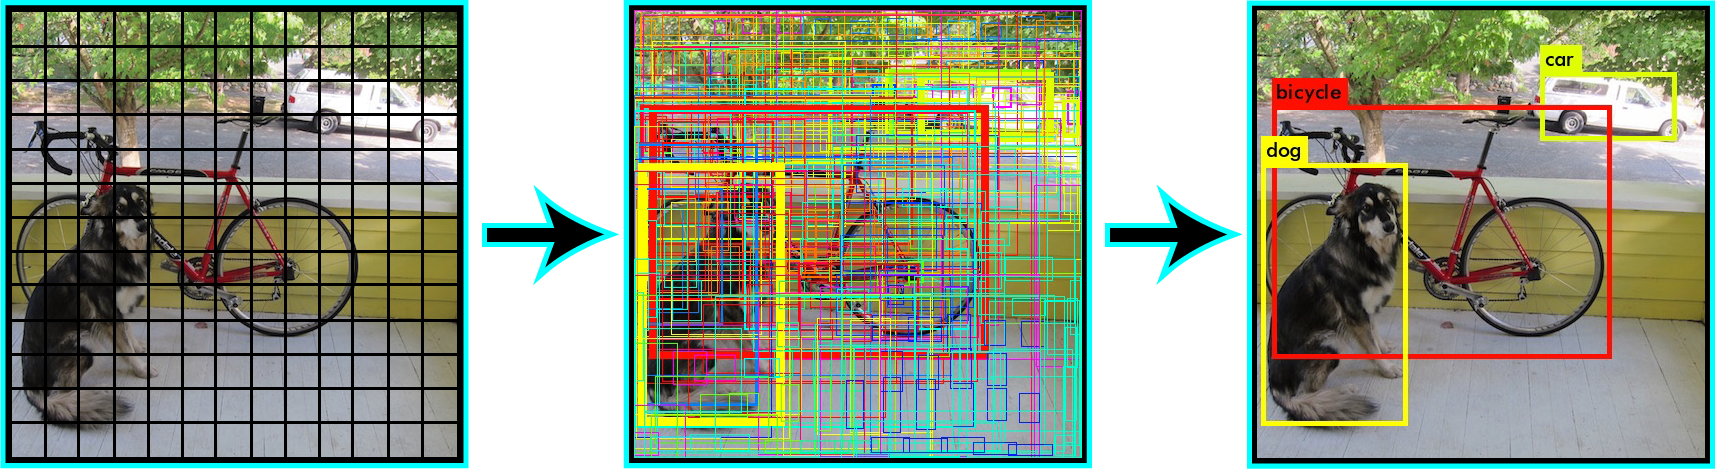
\includegraphics[width=\columnwidth]{./images/yolo.png}
	\caption{The illustration of YOLO}
	\label{yolo}
\end{figure} 
The Alexnet was created in 2012 by Alex Krizhevesky in collaboration with Ilya Sutskever and Geoffrey Hinton. AlexNet won the ImageNet Large Scale Visual Recognition Challenge(ILSVRC) by outperforming all prior competitors. ImageNet \cite{imagenet} is a large database of quality controlled, human-annotated images that help test algorithms that are built to store, retrieve, or annotate multimedia data. Convolutional Neural Networks became the gold standard for image classification after Kriszhevsky's CNN's performance during ImageNet. The convolutional neural networks are slow and expensive in terms of computation. R-CNN solved this problem by reducing the number of bounding boxes that are fed to the classifier \cite{3}. In R-CNN nearly 2000 bounding boxes are fed into the classifier. This selective search method replaces the exhaustive search method which is used to capture object location. After extracting the region proposals \cite{9} it compute the CNN features. Then it classify the regions. The single shot detector(SSD) \cite{ssd} is published in 2015 by Wei Liu et al. The SSD predicts offset of predefined anchor boxes for every location of the feature map. Feature maps at different levels have different receptive field sizes. Here only one feature is responsible for objects at one particular scale. The YOLO (You Only Looks Once) \cite{yolo} is an example of single stage detector. Because it directly predicts the bounding boxes and probability of each class with a single network in a single evaluation. This will improve the detecton speed. Today different versions of YOLO are present. On every upgrade its accuracy and speed is improving.

\section{Methodology}
Social distancing is the best method to prevent the spread of COVID-19. Social distancing is a process of keeping a minimum space between two persons. This will slows down the spread of COVID-19. But people sometimes tend to forget or neglect the restrictions. So this work is focused to provide automated detection of social distance violations in public places using a deep learning model. The deep learning model can be used effectively to detect social distance vioilations in public places.
\par 
Deep learning and computer vision techniques are used in the proposed system. An open sourced object detection network based on YOLOv4 \cite{yolov4} algorithm is used to detect persons from the images/videos. Basically YOLO is a multiclass classification algorithm, which means YOLO is capable of classify more than two classes. But here the system need to detect person class only. So here the YOLO is used to detect all persons \cite{10} from an image. After detecting the results, the coordinate values of the bounding boxes can be used to calculate the distance. 
\par
\begin{figure}[!h]
	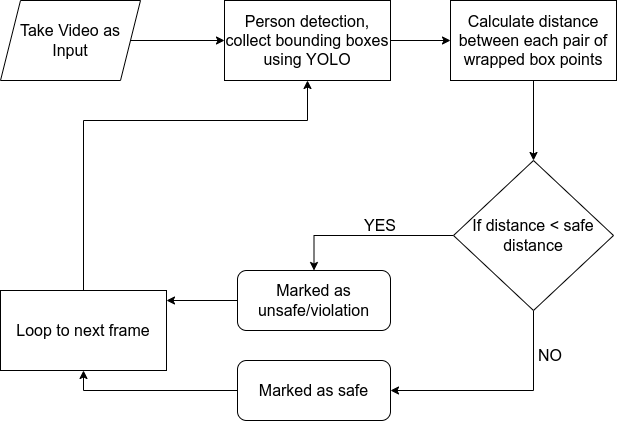
\includegraphics[width=\columnwidth]{./images/flowchart.png}
	\caption{Flowchart of the system}
	\label{pipeline}
\end{figure} 
This system assumes that the pedestrians walks in a flat plane. it is possible to measure the accurate result if the top down view is considered. Before the start of detection, the camera must be calibrated according to the present position. Depending on the distance between two pedestrians the system classifies pedestrians into two classes. One is the class those who are not violating the minimum distance, and the other class is the pair of pedestrians those are violating the minimum distance. The violations are marked in red frame and safe people are marked in green frame. The total number of violations are also calculated. The work was done in Python programming language. The flowchart of this social distance detection system is shown in Fig \ref{pipeline}
\subsection{Pedestrian Detection}
Compared to traditional and machine learning based object detection methods, deep learning based methods reduced the computational complexity issues by formulating the detection with a single regression problem. When considering the the deep learning methods, the YOLO model is considered the best object detectors which can detect objects in real time with high accuracy \cite{yoloreal}. In this work YOLO model is used for pedestrian detection. The YOLO model trained on COCO dataset can able to detect 80 classes including persons. After detecting objects the YOLO model output the object's box coordinates values and corresponding class label. In this work only box coordinate values corresponding to human/pedestrian is used.
\begin{figure}[!h]
	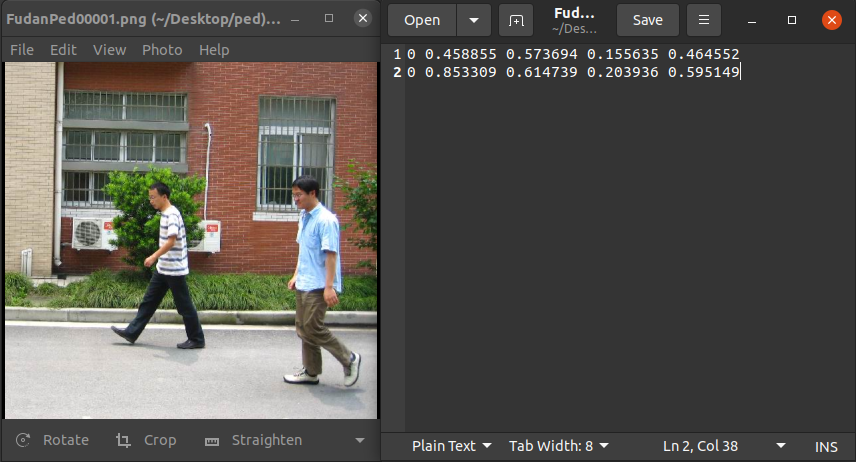
\includegraphics[width=\columnwidth]{./images/dataset.png}
	\caption{Example of dataset}
	\label{dataset}
\end{figure}

\subsection{Distance Measurement}
After the detection of pedestrians from the image, YOLO return the bounding box coordinate values(x,y,w,h). Using these coordinate values, the centre point is calculated. Then the distance between every pedestrian is calculated based on the center point. The distance is scaled by the scaling factor that is estimated from the cameral caliberation. Consider the center point of two pedestrian are $(x_1,y_1)$ and $(x_2,y_2)$ respectively, then the distance (d) between them is calculated using the Euclidean method as 
\begin{equation}
	d = \sqrt{(x_2-x_1)^2+(y_2-y_1)^2}
\end{equation}

\subsection{Classification}
After computing the distance, the next step is classification. This system classify every pedestrians in a frame into two classes. One is people who are following the social distancing and others who are violating the social distancing. In order to decide the violations, a threshold is defined. The threshold is determined according to the cameral caliberation. In this project, the value of the threshold is given as 50 pixels. If the distance between two people is less than this threshold, then these people will classify in unsafe class, otherwise in safe class. The unsafe pair will be marked in red color and the safe pairs will be marked in green color. 
\begin{equation}
	class = \left\{
	\begin{array}{ll}
		safe & d \ge t \\
		unsafe & d < t
	\end{array}
	\right\}
\end{equation}



\section{Result and Discussion}
The image dataset used is the COCO (Common Object in Context) dataset. The COCO dataset is one of the most popular open source object recogintion database used to train deep learning programs. This database includes thousands of images with millions of already labeled objects for training
\begin{figure}[!h]
	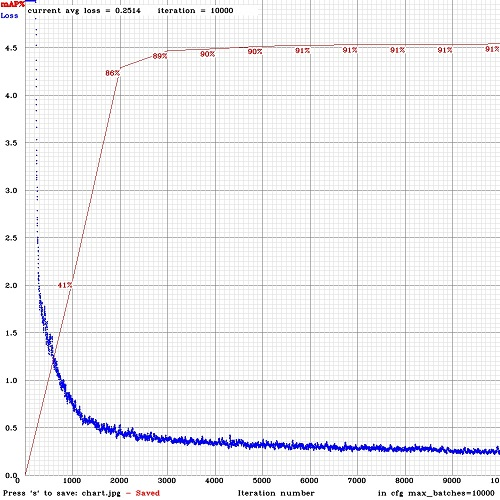
\includegraphics[width=\columnwidth]{./images/loss.jpeg}
	\caption{Loss curve}
	\label{loss}
\end{figure}
An example of a dataset used for this project is shown in Fig \ref{dataset}. In that figure the left side is the image and the corresponding label is in the right side. 
 
Here a video of pedestrians walking on a public street is given as input. The camera is fixed at a specified angle. The distance is defined according to the position of camera. 
\par
Fig \ref{output} shows the social distancing detection in a video frame.The violations are marked in red bounding boxes and safe people are marked in green bounding boxes. If any two bounding boxes overlap each other, then that will also be considered a violation. 
\begin{figure}[!h]
	\centering
	\begin{subfigure}[b]{0.8\columnwidth}
		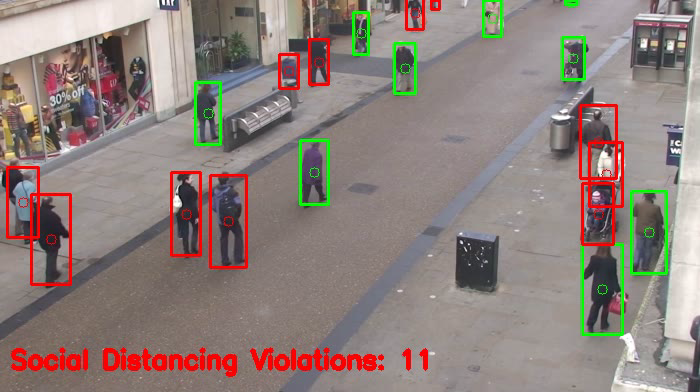
\includegraphics[width=\linewidth]{./images/v1.png}
		\caption{}
	\end{subfigure}
	\begin{subfigure}[b]{0.8\columnwidth}
		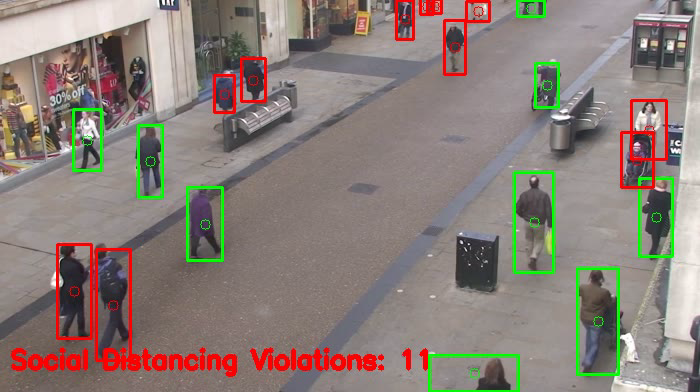
\includegraphics[width=\linewidth]{./images/v2.png}
		\caption{}
	\end{subfigure}
	\begin{subfigure}[b]{0.8\columnwidth}
		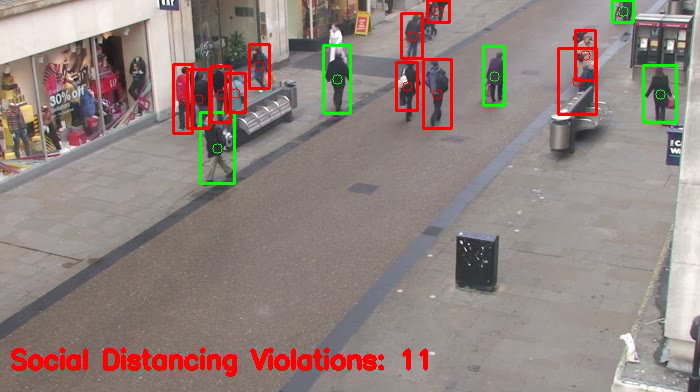
\includegraphics[width=\linewidth]{./images/v4.png}
		\caption{}
	\end{subfigure}
	\caption{Social distance detection in video frame}
	\label{output}
\end{figure}

\par 
YOLO v4 achieves a good results at a real time speed on COCO dataset \cite{coco} with 43.5\% AP running at 65 FPS on Tesla V100. Fig \ref{fps} shows the comparison of YOLOv4 with other models. 

\begin{figure}[!h]
	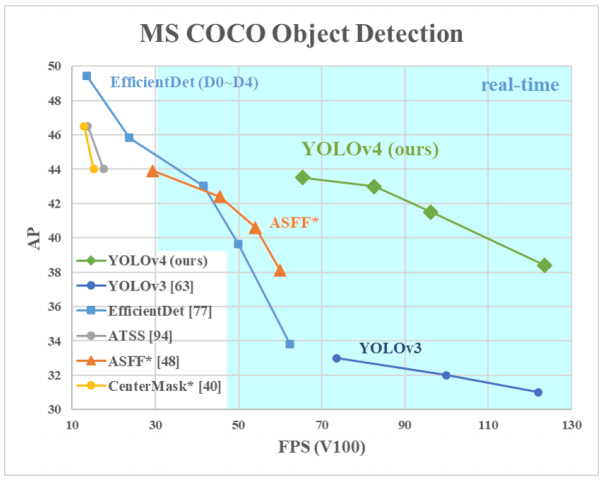
\includegraphics[width=\columnwidth]{./images/fps.png}
	\caption{FPS measured on the Tesla V100 GPU}
	\label{fps}
\end{figure}

Fig \ref{loss} is the loss curve of the model. The blue curve is the training loss or the error on the training dataset. The red line the mean average precision at 50\% Intersection-over-Union threshold (mAP@0.5). There are 600 ground truth and prediction bounding boxes number is 485 and the number of correct predictions is 481. The precision and recall is as follows.
\\
\begin{table}[!h]
	\centering
\begin{tabular}{|c|c|c|c|}
	\hline
	\textbf{Precision} & \textbf{Recall} & \textbf{False Positive Rate} & \textbf{Miss Rate} \\
	\hline
	99.37\% & 80.48\% & 0.63\% & 19.52\% \\
	\hline
\end{tabular}
\caption{Validation Scores}
\label{val}  
\end{table}

\section{Conclusion And Future Works}
A methodology for social distancing detection tools using a deep learning model is proposed. By using computer vision and deep learning, the distance between people can be estimated, and any pair of people who are violating the social distancing will be indicated with a red frame. The proposed method was validated using a video showing pedestrians walking down a street. The visualisation results showed that the proposed method is capable of determining the social distancing measures between people, which can be further developed for use in other environments such as offices, restaurants, and schools.
\par
Furthermore, the work can be further improved by optimising the pedestrian detection algorithm, integrating other detection algorithms such as mask detection and human body temperature detection, improving the computing power of the hardware, and automatic calibration of the camera. 

 
\bibliographystyle{unsrt}

\nocite{*}		

\bibliography{final}		
\hrule
\vspace{.5in}

\end{document}
